% 第二章:导数与微分
\chapter{导数与微分}

\section{导数的定义}

\begin{definition}[导数]
设函数 \( y = f(x) \) 在点 \( x_0 \) 的某个邻域内有定义,当自变量 \( x \) 在 \( x_0 \) 处取得增量 \( \Delta x \)(点 \( x_0 + \Delta x \) 仍在该邻域内)时,相应地函数取得增量 \( \Delta y = f(x_0 + \Delta x) - f(x_0) \)。如果极限
\[ \lim_{\Delta x \to 0} \frac{\Delta y}{\Delta x} = \lim_{\Delta x \to 0} \frac{f(x_0 + \Delta x) - f(x_0)}{\Delta x} \]
存在,则称函数 \( y = f(x) \) 在点 \( x_0 \) 处可导,并称这个极限为函数在点 \( x_0 \) 处的导数,记作 \( f'(x_0) \) 或 \( \left. \frac{\mathrm{d} y}{\mathrm{d} x} \right|_{x = x_0} \)。
\end{definition}

\begin{example}
求函数 \( f(x) = x^2 \) 在 \( x = 1 \) 处的导数。
\end{example}

\begin{solution}
直接求导即可
    \[
f'(1) = \lim_{h \to 0} \frac{f(1+h) - f(1)}{h} = \lim_{h \to 0} \frac{(1+h)^2 - 1}{h} = \lim_{h \to 0} (2 + h) = 2
\]
\end{solution}

\section{微分的定义}

\begin{definition}[微分]
设函数 \( y = f(x) \) 在点 \( x \) 的某个邻域内有定义,如果函数的增量 \( \Delta y = f(x + \Delta x) - f(x) \) 可以表示为
\[ \Delta y = A \Delta x + o(\Delta x) \]
其中 \( A \) 是不依赖于 \( \Delta x \) 的常数,那么称函数 \( y = f(x) \) 在点 \( x \) 处可微,而 \( A \Delta x \) 叫做函数在点 \( x \) 处相应于自变量增量 \( \Delta x \) 的微分,记作 \( \mathrm{d}y \),即 \( \mathrm{d}y = A \Delta x \)。
\end{definition}

% 图片插入示例(注释掉,避免报错)
% \begin{figure}[htbp]
%     \centering
%     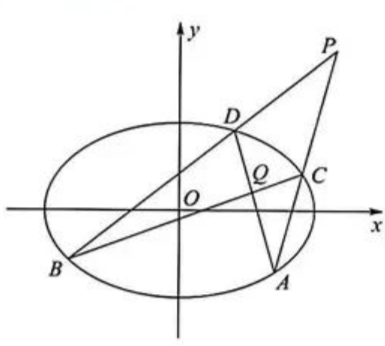
\includegraphics[width=0.6\textwidth]{flg/example.png}
%     \caption{导数的几何意义}
%     \label{fig:derivative}
% \end{figure}